%  Autor: Michael Entrup geb. Epping
%  E-Mail: michael.entrup@wwu.de
%  Version: 1.0.0
%  Datum: Juli 2015
%  Info: Dies is eine einfache Vorlage für das erstellen eines Protokolls.
%		Die Vorlage basiert auf einer Vorlage von Anke B. Schmidt.
%		Sie ist auf die Verwendung im Rahmen der Experimentellen Übungen I im Fachbereich Physik der Uni Münster ausgelegt.
%  Copyright: CC BY 4.0 (http://creativecommons.org/licenses/by/4.0/)

% scrartcl ist die KOMA-Script Variante von article. Für deutsche Texte sollte man generell die Klassen des KOMA-Scriptes verwenden.
\documentclass[
	% Dies sind globale Parameter. Sie gelten für die Dokumentenklasse selbst, aber auch für Pakete, welche später geladen werden. ngerman wird auch dem Paket babel genutzt, weshalb bei diesem kein optionaler Parameter verwendet wird.
	% Schriftgröße
	fontsize=11pt,
	% Papierformat
	paper=a4,
	% schreibt die Papiergröße korrekt ins Ausgabedokument
	pagesize=auto,
	% Normalerweise wird die erste Zeile eines Absatzes eingerückt, um diesen hervorzuheben. Als Alternative kann man parskip aktivieren, womit statt dem Einrücken ein vertikaler Abstand verwendet wird. Typische Werte sind false, half und full.
	parskip=false,
	% Titelseite erzeugen
	titlepage=on,
	% Sprache des Dokuments
	ngerman
]{scrartcl}
% Hier gibt man den Zeichensatz dieser Datei vor (schreibt man mit dem Windows Editor/Notepad, dann muss man hier 'latin1' statt 'utf8' verwenden.
\usepackage[utf8]{inputenc}
% Es werden Schriftarten mit Umlauten verwendet. So ersteint wirklich ein ä in der PDF-Datei und nicht ein a mit hochgestellten Punkten. Dies ist wichtig für die Volltextsuche.
\usepackage[T1]{fontenc}
% Hiermit wird die richtige Silbentrennung aktiviert. Außerdem wird eine passende Darstellung des Datums gewählt. Verwendet man kein KOMA-Script, dann werden auch die sonst englischsprachigen Begriffe, wie scapter, section, appendix usw. ins Deutsche übersetzt. Die in documentclass angegebene Sprache wird auch hier verwendet, falls man keinen optionalen Parameter angibt.
\usepackage{babel}
% Bietet erweiterte Funktionen beim setzten von Formeln (wird z.B. für die align-Umgebung benötigt).
\usepackage{amsmath}
% Schriftart, die am Bildschirm besser lesbar ist.
\usepackage{lmodern}
% Zum Einbinden von Bildern (mehr Dateiformate werden unterstützt).
\usepackage{graphicx}
% Zur Darstellung von Webadressen, E-Mails usw. Besonders praktisch ist, dass man innerhalb von \url{} keine Maskierung verwenden muss: Statt '\_' verwendet man einfach '_'.
\usepackage{url}
% Verbessert den Textsatz. Abstände zwischen Wörtern/Zeichen werden optimiert. Dieses Paket sollte immer zuletzt geladen werden.
\usepackage{microtype}

% Hier werden die Parameter für die Titelseite festgelegt.
% Es wird keine eigene Titelseite gestaltet, sondern der Standard der benutzten Dokumentenklasse verwendet.
% Die Titelseite wird weiter Unten mit \maketitle erzeugt.
\title{Protokoll zu Versuch V1:\\\LaTeX-Vorlage für ein Versuchsprotokoll}
\subtitle{durchgeführt am 08.07.2015 bei Betreuer X Y}
\author{
	% Anders als sonst nutzt man hier das \and für den Zeilenumbruch. \\ kann auch verwendet werden, man sollte nur nicht beides kombinieren.
	Gruppe 01 Mi\and
	Michael Entrup (E-Mail: \url{michael.entrup@wwu.de}) \and
	Max Mustermann (E-Mail: \url{m_must42@wwu.de})
}
\date{\today}

\begin{document}

% Titel (bzw. Titelseite) erzeugen.
\maketitle

% Die Dokumentenklasse Artikel sieht keine separate Seite für den Titel vor.
\newpage

% Inhaltsverzeichnis erzeugen. Als Quelle dient Protokoll.toc. Diese Datei wird automatisch von LaTeX erzeugt.
\tableofcontents

\newpage

Diese Vorlage basiert auf einer Vorlage von Anke B.\ Schmidt\footnote{\url{http://www.uni-muenster.de/Physik.PI/Donath/Studieren/anleitung_experimentelle_uebungen.html}}.

\section{Einführung}

Diese Vorlage soll Ihnen den Einstieg in das Erstellen von Versuchsprotokollen mit \LaTeX\ erleichtern. Da das Internet von Anleitungen zum Erstellen von Dokumenten mit \LaTeX\ nur so wimmelt (man gebe zum Beispiel ``Latex Einführung'' bei einer bekannten Suchmaschine ein), wurde hier bewusst auf weitere Erklärungen verzichtet. Bei Fragen inhaltlicher Art zum Erstellen der Versuchsprotokolle, lesen Sie bitte zunächst den Abschnitt \emph{Versuchsprotokoll} im Kapitel \emph{Hinweise} der Anleitungen zu den Experimentellen Übungen \cite{anleitung}. Weitere Fragen kann Ihr Betreuer beantworten, oder Sie kommen in die Sprechstunde der Praktikumsleiter (\url{http://www.uni-muenster.de/Physik.PI/Donath/Studieren/index.html}).

\section{Durchführung}

\subsection{Einbinden von Abbildungen}

\begin{figure}[htb]
	\centering
	% Keine Angabe der Dateiendung nötig, TeX durchsucht den Ordner, in dem dieser Quelltext liegt
	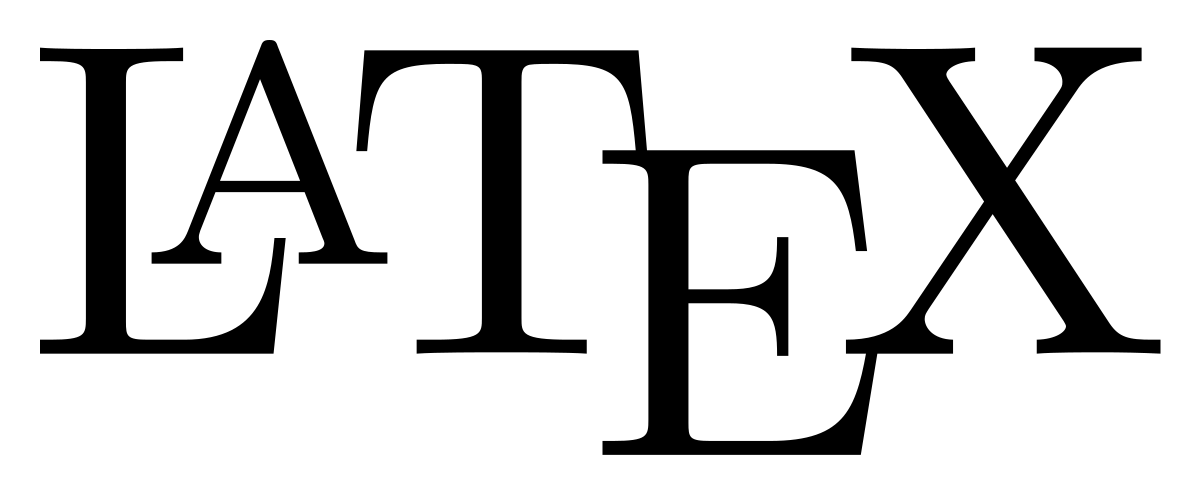
\includegraphics[width=0.6\textwidth]{Bild}
	\caption{Das ist die Bildunterschrift.}\label{Bild}
\end{figure}

Wenn Sie pdf\LaTeX\ verwenden, können Sie Dateien im jpeg-, png-, oder pdf-Format einbinden, wie mit der Abbildung~\ref{Bild} geschehen. \LaTeX\ dagegen erwartet Dateien ausschließlich im eps- oder ps-Format \cite{andyroberts}.

\subsection{Tabellen}

Hier sei auf die einschlägige Literatur verwiesen, zum Beispiel Referenz~\cite{andyroberts} oder Referenz~\cite{hobbits}.

\subsection{Formeln}

Beim Darstellen von Formeln demonstriert \LaTeX\ seine ganze Stärke. Man kann kurze Formeln in den laufenden Text einbinden, zum Beispiel $a^2+b^2=c^2$, den Satz des Pythagoras. Möchte man abgesetzte Formeln verwenden, die durchnummeriert und referenzierbar sind, dann so:
%
\begin{align}\label{formel1}
	\textrm{Student}=\int_\textrm{früh}^\textrm{spät} \mu \; \mathrm{d}e.
\end{align}
%
Auf Formel~(\ref{formel1}), die der geneigte Leser bitte nicht allzu ernst nehmen möge, kann man dann später verweisen.

\section{Diskussion}

Mit Hilfe der zahlreichen Anleitungen, die online zu finden sind, sind Sie sicher bald in der Lage, Ihr Dokument ganz nach Ihren Wünschen zu erweitern und anzupassen. Früher oder später werden Sie auch auf die vielfältigen Möglichkeiten stoßen, das Layout anzupassen. Hierzu möchte ich Ihnen den einleitenden Text zu dem entsprechenden Kapitel aus Referenz~\cite{lshort} mitgeben:
\begin{quote} Chapter 6 contains some potentially dangerous information about how to alter the standard document layout produced by \LaTeX. It will tell you how to change things such that the beautiful output of \LaTeX\ turns ugly or stunning, depending on your abilities.\end{quote}

\begin{thebibliography}{9}

\bibitem{anleitung} Anke B.~Schmidt, \emph{Anleitungen zu den Experimentellen Übungen zur \ldots}.

\bibitem{andyroberts} Andrew Roberts. \emph{Getting to Grips with} \LaTeX, a most useful website: \url{http://www.andy-roberts.net/writing/latex}.

\bibitem{hobbits} Manuela Jürgens und Thomas Feuerstack, \LaTeX\ \emph{-- eine Einführung und ein bisschen mehr \ldots}, FernUniversität in Hagen, Februar 2013.

\bibitem{lshort} Tobias Oetiker, Hubert Partl, Irene Hyna und Elisabeth Schlegl, \emph{The Not So Short Introduction to} \LaTeX\ 2$\varepsilon$.

\end{thebibliography}

\end{document}
